\section{Experiment Setup}
\subsection{Measurement setup and measurement method}
    The measurement setup is shown in Figure \ref{app1}. It consists of a turntable with an integrated photo-gate system used for time measurements.

    Empty turntable is initially rotating and its moment of inertia with respect to the rotation axis is $I_1$. Since the bearings of the turntable are not frictionless, there will be a non-zero frictional torque $M_{\mu}$ causing the turntable to decelerate with angular acceleration $\beta_1$, which can be presented by the following equation,
    \begin{equation}\label{equ_fric}
        M_{\mu}=-I_1\beta_1.
    \end{equation}

    \begin{figure}[H]
    \centering
        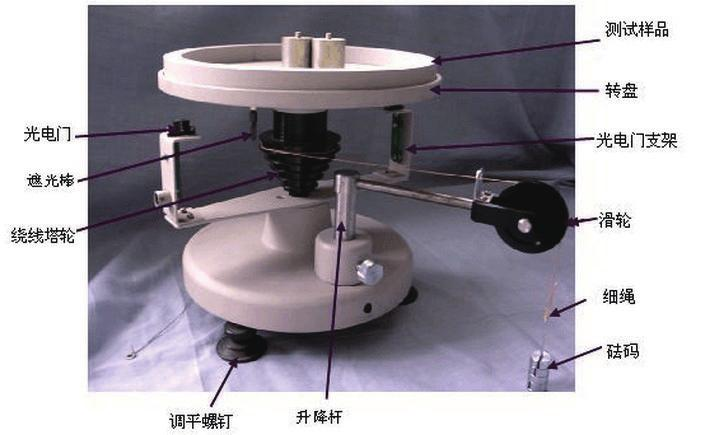
\includegraphics[width=0.7\textwidth]{images/app1}
        \caption{Measurement setup}\label{app1}
    \end{figure}

    Below the turntable, there is a conical pulley of radius R, with a light and inextensible string wound on it. The axis of the cone coincides with the axis of rotation. Attached to the other end of the string passing through a disk pulley, there is a weight with mass $m$, free to move downwards after it is released. If the mass moves downwards with constant acceleration $a$, the tension in the string $T$ is constant and $T=m(g-a)$. If the turntable rotates with angular acceleration $\beta_2$, then $a=R\beta_2$ (we assume that the string does not slip on the pulleys). Hence, the torque is $\tau=TR=m(g-R\beta_2)R$. Consequently, taking into account the frictional torque, the net torque on the turntable is $TR-M_{\mu}$, and the equation of motion for the turntable is
    \begin{equation}\label{equ_motion}
        m(g-R\beta_2)R-M_{\mu}=I_1\beta_2.
    \end{equation}

    Plugging in the Eq.\ref{equ_fric} to Eq.\ref{equ_motion}, we find
    \begin{equation}
        I_1=\frac{mR(g-R\beta_2)}{\beta_2-\beta_1}.
    \end{equation}

    Similarly, we may find the moment of inertia of a rigid body on the turntable by
    \begin{equation}
        I_2=\frac{mR(g-R\beta_4)}{\beta_4-\beta_3}.
    \end{equation}
    where $\beta_3$ is the magnitude of the angular deceleration of the turntable with the body, and $\beta_4$ is its angular acceleration, when the mass m is released and moves downwards.

    Using the fact that the moment of inertia is an additvie quantity, the moment of inertia of the rigid object placed on the turntable, with repect to the axis of the rotation, may be found as the difference
    \begin{equation}\label{equ_I}
        I_3=I_2-I_1.
    \end{equation}
    
\subsection{Measurement of angular acceleration}
    At the edge of the turtable two shielding pins are fixed. The pins will send signals to the photo-gate with the phase interval of $\pi$. An integrated counter-type electronic timer is used to measure the consecutive number $k$ and the time of the photo-gate signal.
    
    If ($k,t$) is a set of the measurement data, the corresponding angular position is
    \[
        \theta=k\pi=\omega_0t+\frac{1}{2}\beta t^2
    \]
    where $\omega_0$ is the initial angular speed. Now, by performing a quadratic fit to the measurement data, we can find the angular acceleration.

\subsection{Devices precision}
    The precisions of the devices are shown in Table \ref{precision}.
    \begin{table}[H]
        \centering
        \begin{tabular}{|l|c|c|}
            \hline
            Devices & Precision & Unit\\ \hline
            Calliper & $2\e{-5}$ & [m]\\ \hline
            Electronic balance & $1\e{-4}$ & [kg]\\ \hline
            Timer & $1\e{-4}\pm0.004\%$ & [s]\\\hline
        \end{tabular}
        \caption{Precision of the measurement instruments}\label{precision}
    \end{table}